\documentclass[12pt,a4paper]{article}
\usepackage[utf8]{inputenc}
\usepackage[T1]{fontenc}
\usepackage{dcolumn}
\usepackage[hidelinks]{hyperref}
\usepackage{amsmath}
\usepackage{amsfonts}
\usepackage{amssymb}
\usepackage[nodisplayskipstretch]{setspace}
\usepackage{float}
\usepackage{graphicx}
\graphicspath{ {./images/} }
\usepackage{natbib}
\usepackage{setspace}
\usepackage{geometry}
%\usepackage[makeindex, toc]{glossaries}
%\makeglossaries
%\newglossaryentry{C}{name={C},description={This represents the cost functions for direct auditing cost for the precise- and vague accounting standards model}}

\begin{document}
	\begin{center}
	\vspace{1em}
	\large{Proposal Master Thesis}\\
	\huge Investor Classification \\ 
	\large \vspace{1em}
	University of Basel\\
	\vspace{4em}
	\large
	Author: \\
	Michael von Siebenthal\\
	\vspace{2em}
	Supervisor: \\
	Prof. Dr. Dietmar Maringer\\
	\vspace{2em}
	\today
	\vspace{3em}
	\end{center}
	\thispagestyle{empty}
	\pagebreak
	\newgeometry{left=2.5cm, right=2.5cm, bottom=2.5cm, top=2.5cm}
	\tableofcontents
	\pagebreak
	\onehalfspacing
	\setlength\abovedisplayskip{2.5pt}
	\setlength\belowdisplayskip{2.5pt}
	
	\section{Overview}
		
	The aim of this Master Thesis will be to analyze to what extent Graph Neural Networks (GNN) and its related methods \citep{kipf2016semi,hamilton2017inductive,velivckovic2017graph,vaswani2017attention} 
	can be applied for bank client classification. GNN methods have proves to be very successful for classification or prediction tasks among others. 
	The advantage of these methods is that they can consider the network structure of a dataset (e.g. social network). This is a valuable feature 
	if one for instance compares it to the capabilities of Convolutional Neural Networks (CNN) which can "only" work with grid structures 
	(e.g. image classification). GNN methods are currently widely used in recommendation systems for social media (e.g. Pinterest, \citet{ying2018graph})
	and could be similarly beneficial for banks when classifying clients. Credit Scoring for instance appears to be an application in which GNN perform 
	very well as shown by \citet{sukharev2020ews}. \\

	\noindent Another interesting application and the focus for this thesis would be to classify bank clients according to their investment preference 
	(e.g. which type of products should be advertised to which client?). This would be especially useful in the retail banking segment where advisors 
	typically cannot know their clients personally due to the large number of clients being serviced. Investor classification is the intended main focus
	of the Master Thesis. \\

	\noindent This topic faces many different hurdles due to the low availability and mostly absence of available bank client data. To the extent 
	possible, appropriate data sets will be retrieved (thus far 1 dataset found). The main difficulty however is to find a dataset which both includes 
	attribute/feature data and the network structure of the customer data. For this reason, mostly methods to create synthetic data will be used to 
	create the dataset for the subsequent simulation/testing. \\

	\noindent In the subsequent sections the provisional outline of the intended Master Thesis is briefly presented. 
	
	\section{Introduction}

	This section will provide an overview of network analysis and its applications (e.g. social network analysis, protein folding (AlphaFold)). 
	In addition, applications of GNN that are specifically relevant for business \& economics are presented which are among others:	
	
	\begin{itemize}
		\itemsep-0.5em
		\item Information flow through organizational charts
		\item Relationships / interdependencies between banks
		\item Compliance tasks 
		\item Client classification
	\end{itemize}
	
	\noindent This section will constitute a smaller portion of the Master Thesis and is meant to provide an introduction to the topic of network 
	analysis, why it is relevant to business and economics and describe what the aim of the Master thesis is.

	\section{Theory}
	
	The following subsections will introduce the theory used in the Master Thesis.

	\subsection{Graph Theory}

	In this section a brief introduction to the most important concepts of graph theory will be given. This section will include the relevant concepts
	which in subsequent chapters will be used to analyze the network for the client classification task. The theory in this sections will be based on
	the book "Networks: An Introduction" by Mark \citet*{Newman2010} and the Stanford open lectures by Prof. Jure Leskovec. 
	
	\subsection{Graph Neural Networks}

	This section will introduce the relevant theory required for Graph Neural Networks. In a first step node embedding strategies such as 
	DeepWalk \citep{perozzi2014deepwalk} and node2vec \citep{grover2016node2vec} are introduced which are useful methods for embedding networks into 
	lower dimensional space. Afterwards it is shown how GNN provide a more general and scalable approach as well as how they can be used for 
	classification tasks (e.g. \citet{kipf2016semi}).

	\subsection{Synthetic Graph Data}

	This section will provide an overview of the theory and approach for the synthetic data generation methods. The method applied will be primarily
	based on the "Multiplicative Attribute Graph" (MAG) model \citep{kim2012multiplicative}. This method allows to create completely synthetic 
	networks incl. node attributes. It also allows for known node embeddings to be used for the network generation process. The benefit of this
	method lies in that it can create networks which resemble real-life network structures, such as social networks. \\

	\noindent As mentioned in section 1, bank client data is most likely not going to be available at a useful scale or form. For this reason 
	synthetic data generation methods will be used. For this reason the following staged approach will most likely be used:

	\begin{enumerate}
		\itemsep-0.5em
		\item Create or use an existing dataset such as the bank dataset by \citet{moro2014data}
		\item Use the MAG model to create network connections between nodes
		\item If necessary grow the network using the MAG model or if available alternative methods. 
	\end{enumerate}
	
	\noindent This methods will be used for synthetic, existing and self created (survey) datasets in order to create the network connections and to 
	derive a sufficiently large data set for the subsequent prediction task. 

	\section{Research Question}

	As shown in the previous section, due to limited data access it will have to be created in large part synthetically. The situation in which the 
	feature data of the clients/nodes is known while the network connections are unknown is of particular interest for this Master Thesis. From a 
	research perspective it is typically relatively feasible to attain feature data of clients related to a topic of interest via surveys among other 
	possibilities. It is however very difficult to in addition also capture the associated network connections in a sensible way. While banks 
	do have a unique advantage in this regard in that they can build network data based on client transactions (e.g. payments), access to such data is
	rarely granted. Rare exceptions are for instance the article by \citet{sukharev2020ews}, where they received access to anonymized bank data for
	developing a credit scoring system. \\

	\noindent This leads to the research question of this Master Thesis:

	\begin{quote}
		\textit{To what extent is partially synthetic network data predictive for bank client classification using Graph Neural Networks?} 
	\end{quote}
	
	\noindent The partial synthetic network data refers to datasets where the feature data is known, while the network connections are synthetically 
	created. Most likely the dataset by \citet{moro2014data} will be used to answer this question. Specifically the accuracy of GNNs will be compared
	to the results of the non-GNN method used by \citet{moro2014data}. \\

	\section{Application}

	An application of GNN which will focus on client classification (investor type) will be presented in this section. As mentioned in section 1, 
	advisors servicing retail clients cannot personally know their clients due to the large volume of clients. For this reason often only generic 
	offers are advertised to this client group. For instance an active investor interested in trading stocks or bonds will most likely be advertised 
	mutual funds. This leads to a mismatch which could be resolved through GNN. In order to test the suitability of GNN, a survey will be conducted 
	with at least 100 participants (preferably many more). The survey will ask participants a list of attribute questions as well as their investor 
	type. The investor types and the attributes will be selected based on existing literature and expert interviews. I have worked for over 10 years 
	as an advisor for a large Swiss bank and have good contacts to conduct expert interviews to accompany the extant literature regarding investor 
	type classification. Once the survey is completed, a network structure using the GAM method will be added to the dataset. The analysis of the 
	application will perform an investor classification task using the collected survey data. It will be interesting to see to what extent the client
	classification task can be performed using the small survey dataset. As the collected survey data will most likely be too small for performing
	a GNN analysis, the network will be grown using the MAG method or an alternative method. If the MAG method is used, the network will be created
	synthetically by using the mean of the survey dataset with regard to the random assignment of the features using Bernoulli trials. 
	
	\subsection{Multiplicative Attribute Graph}

	As described in the previous section, the network will be created using the Multiplicative Attribute Graph method. A crucial ingredient for the 
	graph creation are the affinity matrices. Depending on the link-affinity probability, the resulting network structure can differ significantly. The
	link-affinity matrices provide for an area where the probabilities can on the one hand be set based on theory, they however also allow for 
	simulating different scenarios. The synthetic graph creation is best described using the illustration provided by the authors 
	\citep{kim2012multiplicative}:

	\begin{figure}[h]
		\centering
		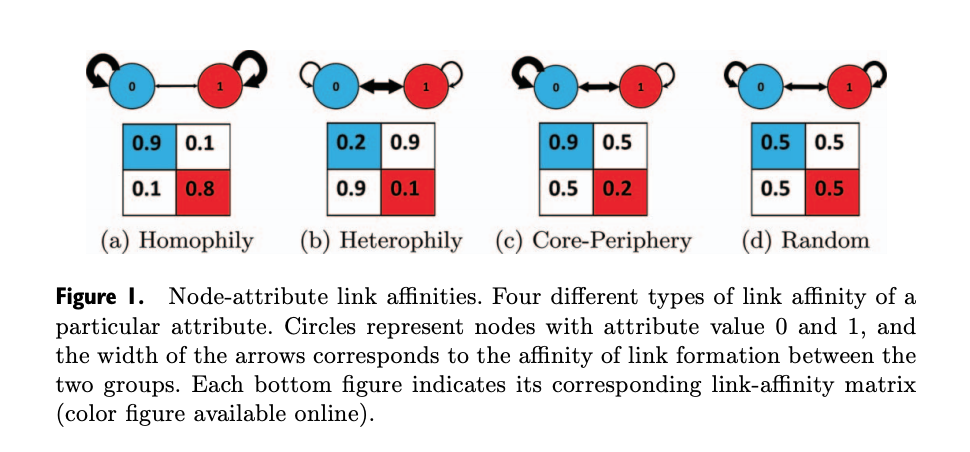
\includegraphics[width=0.8\textwidth]{aff_mat.png}
		\caption{Link-Affinity Matrix}
		\cite{kim2012multiplicative}
		\label{Figure 1}
	\end{figure}

	\begin{figure}[h]
		\centering
		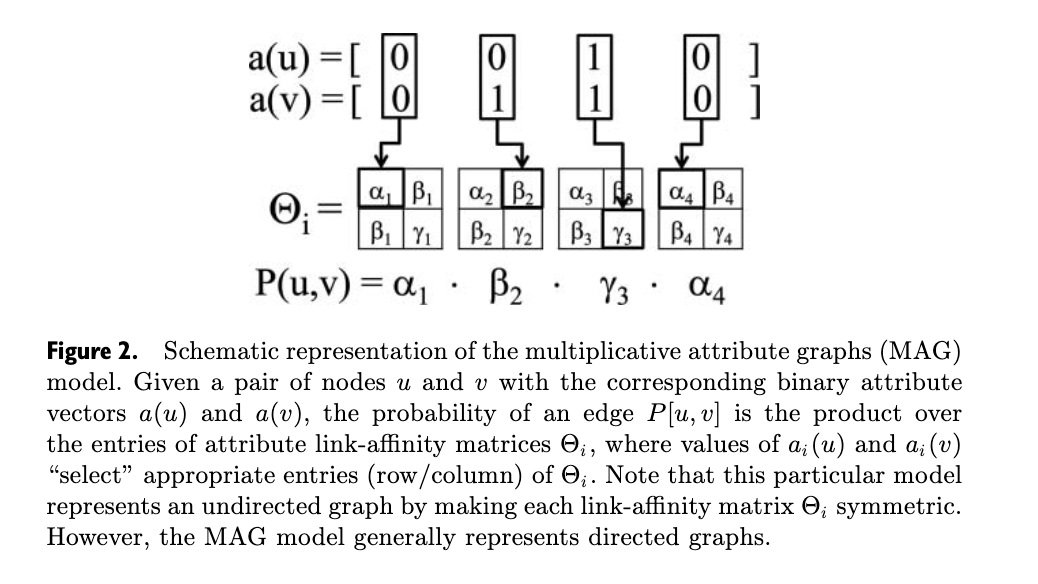
\includegraphics[width=0.8\textwidth]{mag.png}
		\caption{Multiplicative Graph Model}
		\cite{kim2012multiplicative}
		\label{Figure 2}
	\end{figure}
	
	\section{Limitations/Risks}

	The Master Thesis has some limitations and risks regarding myself as the author and the application:

	\begin{enumerate}
		
		\item The topic of GNN is a relatively recent topic and at the limit of my personal programming capabilities. There are fortunately packages
			such as Pytorch Geometric among others which can compensate for some of my programming deficiencies. Nevertheless, even with the support 
			of such packages, the programming skills required is ambitious given the typical programming experience of an economics student. I am
			however confident, that I can successfully complete the project.

		\item The GAM method has shown to create realistic real world networks using attribute data. Nevertheless, this method might fail for 
			analyzing investor types and would negatively impact the accuracy of the GNN.

		\item The survey questionnaire must capture relevant attributes so that the GNN can perform as intended. Failure in this area would negatively
			impact the results. In addition, acquiring sufficient survey participants is a difficult challenge.  

		\item If the GNN does not provide good results, this will put in question the application for which the survey will be conducted. In this case 
			reasons for the failure will be discussed. Further, an alternative classification method will be used for the classification task.

		\item The attractiveness of the Master Thesis relies on the success of the GNN methods chosen. Nevertheless, a failure would point to the 
			limitations of synthetic network creation. Possible reasons for the failure would be researched and discussed which in itself would yield
			useful insights for future research. Nevertheless the aim of the Master Thesis will be to provide a working GNN model.

	\end{enumerate} 

	\pagebreak
	\bibliographystyle{agsm}
	\bibliography{Bibliography}
\end{document}
